% 导言区:设置文档类型和加载需要的宏包
\documentclass[12pt,a4paper]{article} % 使用 article 文档类,字号12pt,纸张A4

% 中文支持
\usepackage[UTF8]{ctex} % 支持中文,编码为 UTF8

% 页面布局设置
\usepackage{geometry} % 控制页面尺寸
\geometry{left=2.5cm, right=2.5cm, top=2.5cm, bottom=2.5cm} % 设置页边距

% 插入图片
\usepackage{graphicx} % 支持插入图片
\usepackage{subcaption} % 支持子图

% 代码高亮
\usepackage{listings} % 插入代码
\usepackage{xcolor} % 定义颜色

% 设置代码样式
\lstset{
    language=C++, % 设置代码语言为 C++
    basicstyle=\ttfamily\small, % 基本字体样式
    keywordstyle=\color{blue}, % 关键词颜色
    commentstyle=\color{gray}, % 注释颜色
    stringstyle=\color{red}, % 字符串颜色
    breaklines=true, % 自动换行
    numbers=left, % 行号位置
    numberstyle=\tiny\color{gray}, % 行号样式
    frame=single, % 代码框
    captionpos=b % 标题位置
}


% 超链接支持
\usepackage[colorlinks, linkcolor=gray,urlcolor=gray]{hyperref} % 设置超链接样式

% 其他常用宏包
\usepackage{amsmath} % 数学公式
\usepackage{amssymb} % 数学符号
\usepackage{booktabs} % 三线表
\usepackage{multirow} % 合并单元格
\usepackage{url} % 支持 \url 命令

% 开始文档
\begin{document}

% 封面部分
\begin{titlepage}
    \centering
    \vspace*{\fill}
    {\Huge \textbf{五子棋程序开发日志}}\\[2cm] % 标题
    {\Large 作者:刘继轩}\\[1cm] % 作者信息
    {\Large 2400017722}\\[1cm] % 
    {最后修改日期:\today}\\[2cm] % 当前日期,自动生成
    \vspace*{\fill}
\end{titlepage}

% 目录
\tableofcontents % 自动生成目录
\newpage

% 日志正文
% 使用 \include 命令引用每日日志文件
% \include 命令会在引用的文件前后自动插入分页符
% 如果不需要分页符,可以使用 \input 命令

% 示例引用两日日志
\section{2024年11月13日} % 日期作为章节显示在目录中

\subsection{今日进展} % 今日进展
今天了解了作业的具体要求,了解了使用C++实现五子棋对弈程序所需要的算法基础,即Min-Max算法和Alpha-Bata剪枝优化。
然后在GitHub上创建了仓库,方便后续的版本控制和更新。并使用GPT生成了latex模板方便后续开发日志的记录。
同时今天找到了一些宝贵的学习参考资源,比如GitHub上基于Javascript语言的五子棋AI教程\url{https://github.com/lihongxun945/gobang?tab=readme-ov-file}和

\subsection{本次作业的基本要求} 

\subsubsection{五子棋详细规则}

黑白双方轮流落子,黑方为先手。

在横、竖、斜方向上连成五子(连续五个棋子皆为己方)者为胜。

黑棋在行棋过程中,如果违反以下“禁手规则”会被判负。

三三禁手:黑棋在一个位置下子后,形成两个或两个以上的活三。活三是指在棋盘上有三个连续的黑子,并且两端都有空位可以继续下子形成五连珠。

四四禁手:黑棋在一个位置下子后,形成两个或两个以上的活四。活四是指在棋盘上有四个连续的黑子,并且至少有一个空位可以继续下子形成五连珠。

长连禁手:黑棋在一个位置下子后,形成六个或更多连续的黑子。

四三禁手:黑棋在一个位置下子后,同时形成一个活四和一个活三。这种情况也被视为禁手。

注意到这里的禁手规则,后续需要特定的函数实现。

\subsubsection{其他要求}
棋盘大小可以自定义,如果要参加Botzone \url{https://botzone.org.cn/} 比赛,则棋盘大小为15*15。

\subsection{算法基础介绍}

Min-Max算法:

五子棋看起来有各种各样的走法,而实际上把每一步的走法展开,就是一颗巨大的博弈树。在这个树中,从根节点为0开始,奇数层表示电脑可能的走法,偶数层表示玩家可能的走法。

那么我们如何才能知道哪一个分支的走法是最优的,我们就需要一个评估函数能对当前整个局势作出评估,返回一个分数。我们规定对电脑越有利,分数越大,对玩家越有利,分数越小,分数的起点是0。

我们遍历这颗博弈树的时候就很明显知道该如何选择分支了:

电脑走棋的层我们称为 MAX层,这一层电脑要保证自己利益最大化,那么就需要选分最高的节点。

玩家走棋的层我们称为MIN层,这一层玩家要保证自己的利益最大化,那么就会选分最低的节点。

而每一个节点的分数,都是由子节点决定的,因此我们对博弈树只能进行深度优先搜索而无法进行广度优先搜索。深度优先搜索用递归非常容易实现,然后主要工作其实是完成一个评估函数,这个函数需要对当前局势给出一个比较准确的评分。




\subsubsection{遇到的问题}
在实现棋子下放功能时,点击事件无法正确获取鼠标位置,导致棋子无法准确放置。

\subsubsection{解决方法}
通过调整事件处理函数,使用相对坐标系计算鼠标点击位置,并将其映射到棋盘格子上,实现了准确放置棋子的功能。

\subsection{代码分析} % 代码分析

\subsubsection{核心算法}


\subsubsection{代码解释}
上述代码实现了五子棋的胜利条件检测,包括横向、纵向以及两种斜向的五子连线检查。

\subsection{明日计划} % 明日计划
计划实现AI对战功能,优化胜利条件检测算法,并进行界面美化。

\subsection{后续待实现的内容} % 心得体会

胜负判断函数;禁手规则判断函数;局势评估函数;

\section{2024年11月27日} % 日期作为章节显示在目录中

\subsection{今日进展} % 今日进展
1. 完成了棋盘初始化、显示、落子验证的实现。

2. 实现了胜负判断逻辑,通过检查横向、纵向、两种斜向的五子连珠状态,判断玩家是否获胜。

3. 实现了黑白棋的交替落子逻辑,并在有效落子后实时更新棋盘。

4. 优化了终端显示,解决了中文输出乱码问题。

\subsection{成果展示} % 成果展示

\subsubsection{程序界面截图}
\begin{figure}[h]
    \centering
    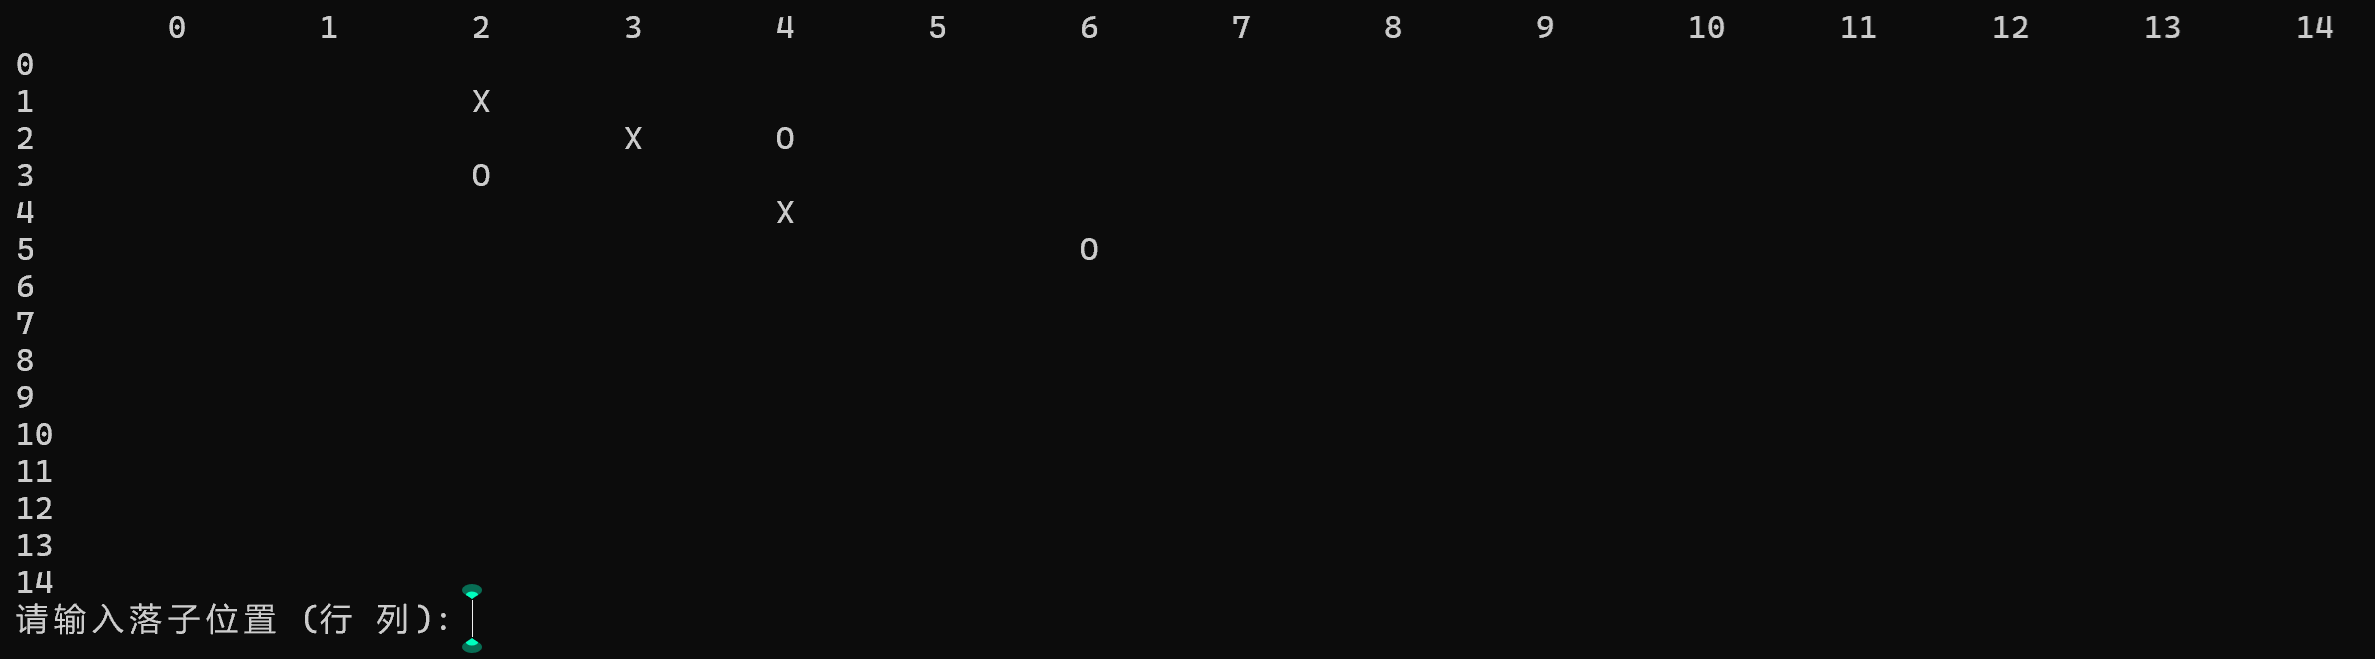
\includegraphics[width=0.7\textwidth]{logs/image/0001.png}
    \caption{程序运行截图}
    \label{fig:program_output}
\end{figure}

\subsubsection{运行结果}
程序成功运行,能够初始化指定大小的棋盘,支持黑白棋交替落子,并正确判断胜负。

\subsection{问题与解决方案} % 问题与解决方案

\subsubsection{遇到的问题}
1. 在终端中显示中文提示时出现乱码。

2. 无法确定落子是否形成五子连珠,导致游戏胜负判断逻辑缺失。

\subsubsection{解决方法}
1. 使用 `SetConsoleOutputCP(65001)` 将控制台编码设置为 UTF-8,解决了中文乱码问题。

2. 编写了 `checkwin` 函数,通过遍历四个方向检查当前玩家是否形成五子连珠。

\subsection{代码分析} % 代码分析

\subsubsection{棋盘初始化与显示}
\begin{lstlisting}[caption={棋盘初始化与显示代码}, label={code:board_init}]
vector<vector<char>> initializeBoard(int size) 
{
    return vector<vector<char>>(size, vector<char>(size, ' '));
}

void displayBoard(const vector<vector<char>>& board) 
{
    cout << "\t";
    for (int i = 0; i < board.size(); ++i) {
        cout << i << "\t";
    }
    cout << endl;

    for (int i = 0; i < board.size(); ++i) {
        cout << i << "\t";
        for (int j = 0; j < board[i].size(); ++j) {
            cout << board[i][j] << "\t";
        }
        cout << endl;
    }
}
\end{lstlisting}

\subsubsection{胜负判断核心代码}
\begin{lstlisting}[caption={五子连珠胜负判断代码}, label={code:win_check}]
bool checkwin(const vector<vector<char>>& board, int x, int y, int currentPlayer) {
    int directions[4][2] = {{1, 0}, {0, 1}, {1, 1}, {1, -1}};
    for (auto direction : directions) {
        int count = 1;

        for (int i = 1; i < 5; i++) {
            int nx = x + i * direction[0];
            int ny = y + i * direction[1];
            if (nx >= 0 && nx < board.size() && ny >= 0 && ny < board.size() && 
                board[nx][ny] == currentPlayerchar[currentPlayer]) {
                count++;
            } else {
                break;
            }
        }
        for (int i = 1; i < 5; i++) {
            int nx = x - i * direction[0];
            int ny = y - i * direction[1];
            if (nx >= 0 && nx < board.size() && ny >= 0 && ny < board.size() && 
                board[nx][ny] == currentPlayerchar[currentPlayer]) {
                count++;
            } else {
                break;
            }
        }
        if (count == 5) return true;
    }
    return false;
}
\end{lstlisting}

\subsection{明日计划} % 明日计划
1. 增加平局检测功能。

2. 实现黑棋禁手规则(如三三禁手、四四禁手)。

3. 为游戏添加菜单功能,支持重新开始或退出。




\section{2024年11月29日} % 日期作为章节显示在目录中

\subsection{今日进展} % 今日进展
1. 禁手规则判断:

   - 实现了五子棋的禁手规则检测,包括四种禁手类型:三三禁手、四四禁手、四三禁手和长连禁手。通过检测棋盘上的活三、活四和长连等棋型,成功防止了 AI 进行禁手操作。

2. 局面评估功能:

   - 完成了初步的局面评估功能,结合禁手规则,能够根据当前棋局对每个落子进行评分,评估玩家的进攻和防守局面。

3. 菜单功能:

   - 实现了一个简单的游戏菜单,允许玩家设置黑棋(X)和白棋(O)的玩家类型(人类或 AI)。通过菜单,玩家可以选择是否开始游戏或退出程序。

4. AI 随机算法:

   - 为 AI 实现了一个简单的随机落子算法,使得 AI 能够在棋盘上随机选择一个空位置进行落子。

5. 输入函数设计:

   - 设计并实现了一个输入函数,方便了后续 AI 模块的接入。输入函数根据玩家类型(人类或 AI)动态选择适当的输入方式,简化了 AI 和人类玩家之间的交互。

\subsection{成果展示} % 成果展示

\subsubsection{程序界面截图}
\begin{figure}[h]
    \centering
    % 插入实际的屏幕截图
    \fbox{\parbox[b][5cm][c]{0.7\textwidth}{\centering 程序界面截图(2024年11月29日)}}
    \caption{程序界面截图(2024年11月29日)}
    \label{fig:program_output}
\end{figure}

\subsubsection{运行结果}
1. 禁手规则检测功能成功运行,能够在 AI 落子时避免三三禁手、四四禁手等情况。

2. 随机 AI 在每轮对局中能够随机选择空位置进行落子,且避免禁手操作。

3. 游戏菜单能够正常运行,玩家能够选择黑棋和白棋的玩家类型,并选择开始游戏或退出程序。

4. 目前,AI 和玩家在同一个棋盘上交替落子,程序能够判断胜负、平局以及禁手,确保游戏规则正常执行。

5. 输入函数已成功集成,允许根据玩家类型选择合适的输入方式,便于后续 AI 模块的接入。

\subsection{问题与解决方案} % 问题与解决方案

\subsubsection{遇到的问题}
1. 禁手规则判断存在逻辑漏洞:

   - 初期禁手规则检测时,发现没有正确处理一些复杂局面,尤其是四四禁手和三三禁手的检测,导致 AI 在某些情况下可能仍会选择禁手棋步。
   
2. AI 决策过于简单:

   - 当前的 AI 只使用随机算法选择棋步,虽然可以避免禁手,但缺乏战略性,导致游戏体验较为简单,缺乏挑战性。

3. 棋盘显示与用户交互较为简单:

   - 当前的程序仅依赖终端输出,缺少图形化界面,用户体验较差。

\subsubsection{解决方法}
1. 禁手规则优化:

   - 对三三禁手和四四禁手的判断进行了优化。通过细化禁手检测函数,增加了对活三和活四的严格检查,确保 AI 在选择棋步时能够避开这些禁手规则。
   
2. AI 改进:

   - 目前的 AI 仍然依赖随机算法,下一步将实现基于局面评估函数的 Minimax 算法,并结合 Alpha-Beta 剪枝提升 AI 的智能程度。

3. 游戏菜单优化:

   - 完成了游戏菜单功能,能够实现玩家与 AI 之间的设置。接下来会考虑实现简单的图形界面,以提高用户体验,使游戏界面更加直观。

4. 输入函数集成:

   - 设计并实现了一个简洁的输入函数,解决了不同玩家类型(人类或 AI)之间的输入方式问题。这个函数简化了后续 AI 模块的接入,使得系统更加灵活。

\subsection{代码分析} % 代码分析

\subsubsection{禁手规则检测代码}
\begin{lstlisting}[caption={禁手规则判断核心代码}, label={code:forbiddenMove}]
bool isForbiddenMove(const vector<vector<char>>& board, int x, int y) 
{
    int liveThreeCount = 0, liveFourCount = 0;

    for (auto dir : directions) 
    {
        if (isLiveThree(board, x, y, 'X', dir[0], dir[1])) liveThreeCount++;
        if (isLiveFour(board, x, y, 'X', dir[0], dir[1])) liveFourCount++;
    }

    // 禁手规则判断
    if (isOverline(board, x, y, 'X')) 
    {
        cout << "长连禁手!" << endl;
        return true;
    }
    if (liveThreeCount >= 2) 
    {
        cout << "三三禁手!" << endl;
        return true;
    }
    if (liveFourCount >= 2) 
    {
        cout << "四四禁手!" << endl;
        return true;
    }
    if (liveThreeCount >= 1 && liveFourCount >= 1) 
    {
        cout << "四三禁手!" << endl;
        return true;
    }

    return false; // 没有禁手
}
\end{lstlisting}

\subsubsection{菜单功能代码}
\begin{lstlisting}[caption={游戏菜单功能代码}, label={code:menu}]
void displayMenu(bool &blackPlayerType, bool &whitePlayerType)
{
    cout << "====五子棋游戏菜单====" << endl;
    cout << "1.设置玩家类型" << endl;
    cout << "2.开始游戏" << endl;
    cout << "3.退出游戏" << endl;

    int choice = -1;

    while(true)
    {
        cout << "请选择:" << endl;
        cin >> choice;
        switch(choice)
        {
            case 1:
                cout << "选择黑棋(X)玩家类型:" << endl;
                cout << "1.人类玩家" << endl;
                cout << "2.AI 玩家" << endl;
                int blackChoice;
                cin >> blackChoice;
                blackPlayerType = (blackChoice == 1) ? false : true;
                cout << "选择白棋(O)玩家类型:" << endl;
                cout << "1.人类玩家" << endl;
                cout << "2.AI 玩家" << endl;
                int whiteChoice;
                cin >> whiteChoice;
                whitePlayerType = (whiteChoice == 1) ? false : true;
                break;
            case 2:
                cout << "开始游戏..." << endl;
                return; // 返回,开始游戏
            case 3:
                cout << "退出游戏..." << endl;
                exit(0); // 退出程序
            default:
                cout << "请重新选择!" << endl;
        }
    }
}
\end{lstlisting}

\subsubsection{输入函数代码}
\begin{lstlisting}[caption={输入函数设计}, label={code:inputFunction}]
void processInput(const string& playerType, const vector<vector<char>>& board, char currentPlayer) {
    if (playerType == "human") {
        manualInput(board);
    } else if (playerType == "ai") {
        aiInput(board);
    }
}

void manualInput(const vector<vector<char>>& board) {
    int x, y;
    cout << "请输入落子位置 (行 列): ";
    cin >> x >> y;
    // 检查位置有效性
}

void aiInput(const vector<vector<char>>& board) {
    // 简单随机AI输入
    srand(time(0)); // 随机种子
    int x = rand() % board.size();
    int y = rand() % board.size();
    cout << "AI 选择位置: (" << x << ", " << y << ")" << endl;
}
\end{lstlisting}

\subsection{明日计划} % 明日计划
1. 完善 Minimax 算法,结合 Alpha-Beta 剪枝提升 AI 智能,减少计算时间。

2. 实现 AI 基于评估函数的决策逻辑,替代随机算法,提升游戏体验。

3. 开始实现简单的图形化界面,展示棋盘、玩家及AI的落子。

4. 优化 禁手检测,确保所有禁手类型都能被准确识别并避免。



% 引用 日志


% 如果日志内容较多,可以继续添加 \include 命令引用更多日志文件

% 参考文献
\begin{thebibliography}{9} % 参考文献列表
\bibitem{ref1} 作者, \textit{书名}, 出版社, 出版年份.
\bibitem{ref2} 在线资源标题, \url{https://example.com}
\end{thebibliography}

\end{document}
